% !TeX encoding = UTF-8
% Inicio% Inicio

\documentclass[xcolor=dvipsnames]{beamer}
\usetheme[left,width=1.8cm, hideothersubsections,numbers,totalnumber,compress,sidebarshades]{PaloAlto}
\setbeamertemplate{footline}[frame number]
\setbeamertemplate{navigation symbols}{}
\setbeamertemplate{items}[ball]
\setbeamertemplate{blocks}[rounded][shadow=true]

\usefonttheme{professionalfonts}% font de LaTeX
\useinnertheme{rounded}

% Colores
\definecolor{micolor}{rgb}{0.25,0.1,0.25}
\usecolortheme[named=micolor]{structure} % violet
\setbeamercolor{normal text}{bg=violet!5,fg=black}

\setbeamercolor*{palette primary}{use=structure,fg=micolor,bg=micolor!10}
\setbeamercolor*{sidebar}{use=structure,fg=micolor,bg=,bg=micolor!10}

\setbeamercolor*{palette sidebar primary}{use=structure,fg=micolor} 
\setbeamercolor*{palette sidebar secondary}{use=structure,fg=micolor} 
\setbeamercolor*{palette sidebar tertiary}{use=structure,fg=micolor} 
\setbeamercolor*{palette sidebar quaternary}{use=structure,fg=micolor} 
\setbeamercolor*{page number in sidebar}{fg=micolor}

\setbeamercolor*{titlelike}{use=structure,fg=white, bg=micolor}

\setbeamercolor{block title}{use=structure,fg=white,bg=structure.fg!75!black} 

\logo{\incsvg{1.8cm}{EHU}}
\setbeamercolor{logo}{fg=black,bg=micolor!10}

% Paquetes

\usepackage[spanish]{babel}     % Paquete de lenguaje español
\usepackage[utf8]{inputenc}
%\usepackage[latin1]{inputenc}
\usepackage{amsmath}
\usepackage{amssymb}
\usepackage{color,graphicx}
\usepackage{eurosym}

\usepackage{latexsym} % Simbolos
\usepackage{colortbl}%soporte para color en tablas
\usepackage{euro}
\usepackage{natbib}
\bibliographystyle{plainnat}

%  Hace saltar una línea entre párrafos
% \addtolength{\parskip}{\baselineskip}
%  Hace saltar unos puntos entre párrafos
% \addtolength{\parskip}{5pt}
\addtolength{\parskip}{5pt}
%\usepackage{garamond}          % Usar tipo
%\usepackage[urw-garamond]{mathdesign}
\usepackage{libertine} 
%usepackage[libertine]{newtxmath}
%\usepackage{bera}


% para tt
\usepackage{courier}


\usepackage{listings}
\lstset{
    language=bash, %C, % Octave -> choose the language of the code
    basicstyle=\scriptsize \ttfamily\bfseries, %  -> the size of the fonts used for the code
    %     basicstyle=\small\ttfamily, %  -> the size of the fonts used for the code
%    numbers=left, %  -> where to put the line-numbers
%    numberstyle=\tiny, %  -> size of the fonts used for the line-numbers
%    stepnumber=3, %  -> the step between two line-numbers.
%    numbersep=5pt, %  -> how far the line-numbers are from the code
%    backgroundcolor=\color{white}, %  -> sets background color (needs package)
    showspaces=false, %  -> show spaces adding particular underscores
    showstringspaces=false, %  -> underline spaces within strings
    showtabs=false, %  -> show tabs within strings through particular underscores
    %     frame=single, %  -> adds a frame around the code
%    frame=ltrb,framesep=2pt, % Left,Top,Right,Bottom
    tabsize=4, %  -> sets default tab-size to 2 spaces
    captionpos=b, %  -> sets the caption-position to bottom
    breaklines=true, %  -> sets automatic line breaking
    breakatwhitespace=false, %  -> automatic breaks happen at whitespace
    %     morecomment=[l]{//}, %  -> displays comments in italics (language dependent)
    %     frame=shadowbox, % draw a frame around your source code with a blue shadow
    %     rulesepcolor=\color{blue}, % draw a frame around your source code with a blue shadow
    % frame=ltrb,framesep=5pt,
    keywordstyle=\ttfamily\bfseries\color{blue},
    identifierstyle=\ttfamily\color{black},
    commentstyle=\itshape\color{ForestGreen},
    stringstyle=\ttfamily\color{red},
}


\def\newblock{}

\usepackage{url}
\def\R2Lurl#1#2{\mbox{\href{#1}{\color{blue}\ttfamily #2}}}

% % % % % % Para imprimir 2 pantallas en una directamente
% \usepackage{pgfpages}
% \pgfpagesuselayout{2 on 1}[a4paper,border shrink=5mm]
% \pgfpagesuselayout{4 on 1}[a4paper,border shrink=5mm, landscape]
% \mode<handout>{\setbeamercolor{background canvas}{bg=black!5}}
% Para imprimir varias en una
% \usepackage{pgfpages}
% \pgfpagesuselayout{8 on 1}[a4paper,border shrink=5mm]
% \pgfpagesuselayout{4 on 1}[a4paper,border shrink=5mm, landscape]
% \pgfpagesuselayout{2 on 1}[a4paper,border shrink=5mm]
% % % % % % Para imprimir 2 pantallas en una directamente

% \usepackage{pgfpages}
% \mode<presentation>
% {
% %  % \usetheme{default}
% %   \usetheme{progressbar}
%   \pgfpagesuselayout{4 on 1}[a4paper, landscape, border shrink=3mm]
% }

\newcommand{\Rojo}{ {\color{red} TODO: } }
\newcommand{\tab}{\hspace{5mm}}

% Título
\newcommand{\titulo}{\texttt{Vagrant} y \texttt{Docker}}



\definecolor{purple}        {cmyk}{0.45, 0.86, 0   , 0   }

\hypersetup{
	linkcolor=blue,citecolor=purple,pagecolor=red,urlcolor=blue, anchorcolor = red
}
\hypersetup{
	pdfborder={0 0 0}
}

% % rellenamos la info del fichero PDF
\hypersetup{
	pdftitle =
	\titulo,
	pdfauthor =
	Pablo González Nalda (http://lsi.vc.ehu.es/pablogn/),
	pdfsubject=
	\titulo,
	pdfkeywords =
	Sistemas Operativos
}

%%%%%%%%%%%%%% SVG
%\include{svg}

%\newcommand{\executeiffilenewer}[3]{%
%	\ifnum\pdfstrcmp{\pdffilemoddate{#1}}%
%	{\pdffilemoddate{#2}}>0%
%	{\immediate\write18{#3}}\fi%
%}


% basado en 
%How to include an SVG image in \LATEX de Johan B. C. Engelen
% Insertar en bash y hacer svgtex cada vez que se añada un svg a la carpeta
%svgtex(){
%	for i in *.svg
%	do
%	inkscape -z -D --file=$i --export-pdf=${i%.*}.pdf --export-latex
%		done
%}

\newcommand{\includesvg}[1]{%
	%	\executeiffilenewer{#1.svg}{#1.pdf}%
	%	{
	%		inkscape -z -D --file=#1.svg --export-pdf=#1.pdf --export-latex
	%		}%
	\input{#1.pdf_tex}%
}

\newcommand{\incsvg}[2]{
	\def\svgwidth{#1}
	\input{#2.pdf_tex}
}


\begin{document}
	% \title[]{Navegación}
	\title[]{\titulo, 2017}
	\subtitle{Toma de contacto}
	
	\author{Pablo González Nalda}
	% \logo{\includegraphics[scale=0.13]{logoEHU}}
	\logo{\incsvg{1.6cm}{EHU}}
	\institute[LSI]{Depto. de Lenguajes y Sistemas Informáticos}
	% \date{\today}
	\date{Febrero de 2017}
	
	% \begin{frame}[plain]
	% \href{run:kk.avi}{videolink}
	% % 	\begin{center}
	% % 		\begin{figure}[ht]
	% % 			\includemovie[ poster, % shows initial frame before play begins controls
	% % 			, % controls are only available on a Mac (they will not appear on windows.)
	% % 			% (if no controls are used, then you can double click the movie to start it.)
	% % 			repeat, % repeat the movie over and over.
	% % 			text=(Loading movie...) % text shown while loading movie
	% % 			]{6cm}{6cm}{kk.avi}
	% % 		\end{figure}
	% % 	\end{center}
	% \end{frame}
	
	\begin{frame}[plain]
		\begin{columns}[c]
			\begin{column}[t]{7.9cm}
				\begin{figure}
					\begin{center}
						\incsvg{3.5cm}{EHU}\hfill
						\incsvg{3cm}{EUI}
					\end{center}
				\end{figure}
				\titlepage
				\begin{center}
					\textit{\tiny Modificado el \today}
				\end{center}
			\end{column}
			\begin{column}[t]{1.8cm} % para centrar la pág de título es como la anchura del usetheme
				\begin{figure}[b]
					\vskip 6cm
					\begin{center}
						\R2Lurl{http://creativecommons.org/licenses/by-sa/2.5/es/}{\incsvg{1.8cm}{CC-logo}}
						\\ \vskip 0.5cm
						\R2Lurl{http://creativecommons.org/licenses/by-sa/2.5/es/}{\incsvg{1.8cm}{ccbysa}}
					\end{center}
				\end{figure}
			\end{column}
		\end{columns}
	\end{frame}
	\author{\scshape Contenidos}
	
	\begin{frame}
			\frametitle{Contenidos de la presentación}
				\tableofcontents[
					% ...showing the active section in the context of other sections...
					sectionstyle=show/show,
					% ... while hiding subsections
					subsectionstyle=hide/hide/hide
				]
	\end{frame}
	
	\AtBeginSection[] {
		%                 \begin{frame}[plain]
		% 				Sección \thesection{}
		%                 \end{frame}
		\begin{frame}
			%                         \frametitle{
			%                                 % Put in the section number
			%                                         \sectionname{} \thesection{}%:
			%                                 % Now also put in the section description
			%                          %            [description]
			%                                 }
			% Generate the table of contents...
			\tableofcontents[
			% ...showing the active section in the context of other sections...
			sectionstyle=show/shaded,
			% ... while hiding subsections
			subsectionstyle=hide/hide/hide
			]
		\end{frame}
	}

% % % % % % % % % % % % % % % % % % % % % % % % % % % % % % % % % % % % % % % % % % %

% % % % % % % % % % % % % % % % % % % % % % % % % % % % % % % % % % % % % % % % % % %

% % % % % % % % % % % % % % % % % % % % % % % % % % % % % % % % % % % % % % % % % % %

% % % % % % % % % % % % % % % % % % % % % % % % % % % % % % % % % % % % % % % % % % %

%\lstinputlisting{senales.c}


%	Aislamiento de subsistemas y contenedores




\section{Objetivos del taller}
\begin{frame}[fragile]
	\frametitle{Objetivos del taller}

En este taller vamos a ver las potencialidades den \texttt{Vagrant} y \texttt{Docker}, que nos permiten:
		\begin{itemize}
			\item Virtualización.
			\item Automatización.
		\end{itemize}
	
	El ejemplo está basado en \url{https://www.sitepoint.com/vagrantfile-explained-setting-provisioning-shell/} con los ejemplos en \url{https://github.com/sitepoint-editors/vagrant-base-config}

\end{frame}

\section{Automatización de la virtualización}
\begin{frame}[fragile]
	\frametitle{Automatización de la virtualización}
	
	Gestión automatizada de máquinas virtuales mediante \texttt{scripts} con \texttt{Vagrant}, que nos permite:
	\begin{itemize}
		\item Crear y destruir máquinas virtuales a través de un fichero de configuración \texttt{Vagrantfile}.
		\item Se usan máquinas genéricas preparadas como base.
		\item Al arrancar se \textit{\textbf{provisionan}} con otro \texttt{script}, que instala, configura y ejecuta los programas adecuados para dar el servicio objetivo de la máquina.
	\end{itemize}
	
	\begin{lstlisting}
vagrant up
vagrant ssh
vagrant destroy
	\end{lstlisting}
	
	Se puede comprobar que son sistemas distintos con \texttt{uname} dentro y fuera de la máquina. La virtualización es a nivel hardware.
\end{frame}

\section{Ventajas de la gestión con máquinas virtuales}
\begin{frame}[fragile]
	\frametitle{Ventajas de la gestión con máquinas virtuales}

Gestionar un sistema con máquinas virtuales nos permite:
		\begin{itemize}
			\item diferenciar los sistemas y los recursos necesarios para proporcionar un servicio: cada sistema es una simulación de ordenador, un SO independiente.
			\item por lo que un problema en una MV sólo va a afectar a un servicio
			\item la creación es repetible y automatizable.
		\end{itemize}
\end{frame}

\section{\texttt{chroot}}
\begin{frame}[fragile]
	\frametitle{\texttt{chroot}}
	\texttt{chroot} es un mecanismo que ejecuta un programa cambiando la raíz de su sistema de ficheros a un directorio, por lo que ese programa puede ser el que arranque un sistema completo. 

	Sólo compartirá con el anterior el sub-árbol de directorios y el kernel. 

	Se pueden montar los subdirectorios especiales como \texttt{/proc}

\end{frame}

\begin{frame}[fragile]
	\frametitle{Ejemplo de uso de \texttt{chroot}}
	Como \texttt{root}
	\begin{lstlisting}
mkdir jaula
cd jaula/
cp /bin/busybox .
./busybox ls
./busybox uname  -a
ldd busybox
mkdir proc dev run var
mount --bind /proc proc # directorio /proc disponible en la jaula
mount --bind /dev dev 
chroot /home/pablo/jaula ./busybox ash
# En otra terminal
sudo ls -ld /proc/18582/root
lrwxrwxrwx 1 root root 0 abr 20 19:56 
              /proc/18582/root -> /home/pablo/jaula
	\end{lstlisting}
Más ejemplos en {\small \url{http://www.cyberciti.biz/faq/unix-linux-chroot-command-examples-usage-syntax/}}
\end{frame}





\section{Mecanismos de aislamiento}
\begin{frame}[fragile]
	\frametitle{Mecanismos de aislamiento: \textit{Namespaces}}

{\scriptsize \url{https://docs.docker.com/engine/understanding-docker/} }

Docker usa diferentes mecanismos proporcionados por el kernel y construidos sobre él. Usa los \texttt{namespaces} para crear entornos aislados en el sistema, los contenedores. Cada elemento del contenedor se ejecuta en su propio \textit{espacio de nombres} y no tiene acceso al exterior.

Algunos de los espacios de nombres que usa Docker son:
		\begin{itemize}
			\item \textbf{pid} namespace: Process isolation (PID: Process ID).
			\item \textbf{net} namespace: Managing NETwork interfaces.
			\item \textbf{ipc} namespace: Managing access to IPC resources (IPC: InterProcess Communication).
			\item  \textbf{mnt} namespace: Managing MouNT-points .
			\item \textbf{uts} namespace: Isolating kernel and version identifiers. (UTS: Unix Timesharing System).
		\end{itemize}
\end{frame}

\begin{frame}[fragile]
	\frametitle{Mecanismos de aislamiento: \textit{Control groups}}

Los \texttt{cgroups} o \textit{grupos de control} controlan la cantidad de recursos que consume el contenedor. De esta forma los contenedores comparten los recursos de hardware y tienen un límite, por ejemplo de memoria disponible. Controlan:
		\begin{itemize}
			\item Limitación de recursos.
			\item Control de prioridades.
			\item Contabilidad.
			\item Control de grupos de procesos (congelar y rearrancar).
		\end{itemize}


\end{frame}

\begin{frame}[fragile]
	\frametitle{Mecanismos de aislamiento \textit{Union file systems}}

Un sistema de ficheros \textit{Union} es el que compone, une la información de varios sistemas de ficheros (las capas) para obtener uno. Esas capas son las fases de creación del sistema de ficheros del contenedor. Las capas pueden ser compartidas por varios contenedores (como el sistema operativo base).


	\begin{lstlisting}
ls -l /var/lib/docker/overlay/
	\end{lstlisting}

\begin{figure}
\centering
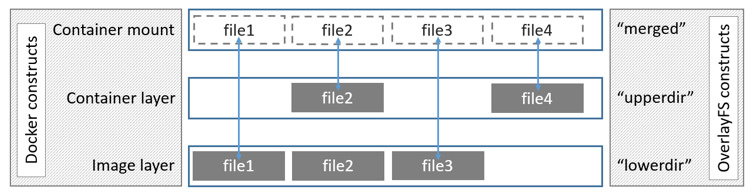
\includegraphics[width=\linewidth]{./overlay_constructs}
\label{fig:overlay_constructs}
\end{figure}

\url{https://docs.docker.com/engine/userguide/storagedriver/overlayfs-driver/}

\end{frame}


\section{Docker}
\begin{frame}[fragile]
	\frametitle{¿Qué es Docker?}
	Docker es un mecanismo para aislar, gestionar y modularizar la ejecución de un servicio, sus procesos y recursos necesarios, como almacenamiento, redes y otros dispositivos.

		\begin{columns}[c]
			\begin{column}[t]{5cm}
				\begin{figure}
					\begin{center}
\centering
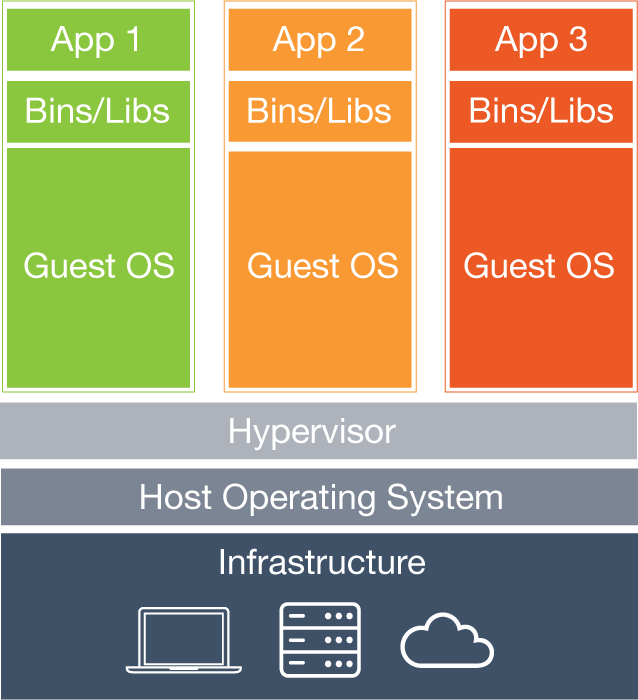
\includegraphics[width=0.7\linewidth]{./what-is-docker-diagram}
\caption{Virtualización a nivel de hardware}
\label{fig:what-is-docker-diagram}
					\end{center}
				\end{figure}
			\end{column}
			\begin{column}[t]{5cm}
				\begin{figure}[b]
					\vskip 1.35cm
					\begin{center}
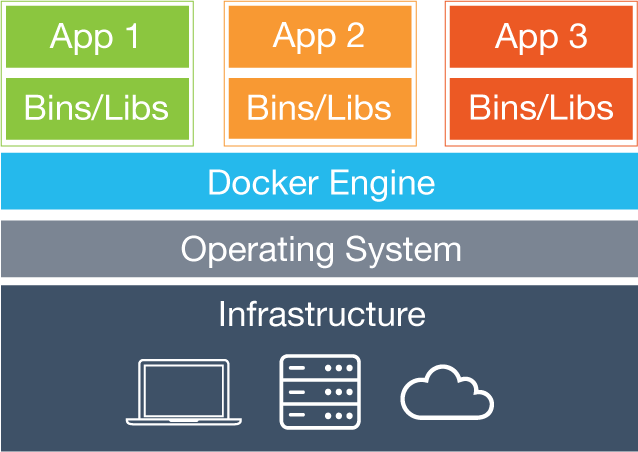
\includegraphics[width=0.7\linewidth]{./what-is-vm-diagram}
\caption{Contenedores}
\label{fig:what-is-vm-diagram}
					\end{center}
				\end{figure}
			\end{column}
		\end{columns}

\end{frame}


\begin{frame}[fragile]
	\frametitle{Estructura de un contenedor}

	Un contenedor comparte el kernel con el resto de procesos del sistema, puesto que el contenedor aísla servicios formados por varios procesos que colaboran. Se puede distinguir 
	\begin{description}[contenedor]
		\item [imagen] el conjunto de capas de sólo lectura que forman el sistema de ficheros
		\item [contenedor] una imagen con una capa de lectura y escritura
	\end{description}

	Cuando hablamos de SO, pensamos en el conjunto de ficheros y mecanismos básicos para arrancar en el contenedor los servicios necesarios para un programa estándar de ese sistema. Sin embargo, el contenedor no arranca ningún proceso.

\end{frame}


\begin{frame}[fragile]
	\frametitle{Estructura de un contenedor}

		\begin{columns}[c]
			\begin{column}[t]{6cm}
			~\\
Cada capa (\textit{image-layer}) es un sistema de ficheros de sólo lectura, y es el resultado de una fase de instalación de software. Las capas se unen con un sistema de ficheros de \texttt{UnionFS}. Cuando arranca el contenedor se añade una capa vacía de escritura.
			\end{column}
			\begin{column}[t]{4cm}
				\begin{figure}
					\begin{center}
\begin{figure}
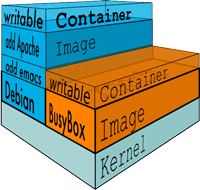
\includegraphics[width=\linewidth]{./what_is_layered_filesystems_sm}
\label{fig:what_is_layered_filesystems_sm}
\end{figure}
					\end{center}
				\end{figure}
			\end{column}
		\end{columns}
\begin{figure}
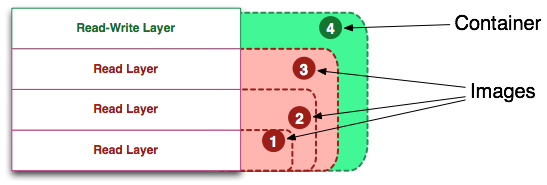
\includegraphics[width=0.7\linewidth]{capas}
\label{fig:capas}
{\tiny \url{http://merrigrove.blogspot.com.es/2015/10/visualizing-docker-containers-and-images.html} }
\end{figure}
\end{frame}

\begin{frame}[fragile]
	\frametitle{Estructura de un contenedor}

			Docker ejecuta un programa confinando ese proceso en 
			
\begin{itemize}
	\item 	un juego de PIDs separados, 
	\item con sistemas de ficheros propio, 
	\item volúmenes propios montados
	\item  y acceso a una red definida por software.
\end{itemize}
			
		
\end{frame}

\begin{frame}[fragile]
	\frametitle{\texttt{docker pull ros}}
		\begin{lstlisting}

$ docker pull ros
Using default tag: latest
latest: Pulling from library/ros
203137e8afd5: Pull complete 
2ff1bbbe9310: Pull complete 
933ae2486129: Pull complete 
a3ed95caeb02: Pull complete 
efa7035358b8: Pull complete 
492b493cc7ff: Pull complete 
b95358183d2d: Pull complete 
103c3645b87a: Pull complete 
1cd6ee992a45: Pull complete 
1fc2ba02a5ca: Pull complete 
6eec5fc93cc9: Pull complete 
f580de0c172a: Pull complete 
Digest: sha256:078fbd221da8a3126eff2e2836572e38ef94631a1017568b86
Status: Downloaded newer image for ros:latest

		\end{lstlisting}
\end{frame}


\begin{frame}[fragile]
	\frametitle{Otras instrucciones básicas}
		\begin{lstlisting}
$ docker run -it bitnami/minideb touch hola       
Unable to find image 'bitnami/minideb:latest' locally
latest: Pulling from bitnami/minideb
15abd30c6809: Pull complete 
Digest: sha256:07dbd4421b362a5d33665b868fb0dde89e06437905e04cc85f00e6bb862d68a8
Status: Downloaded newer image for bitnami/minideb:latest

$ docker images  # sistema de ficheros en capas + def. de recursos
$ docker ps 	 # instancias en funcionamiento, contenedores
$ docker ps -a   # instancias en funcionamiento y paradas

		\end{lstlisting}
\end{frame}

\begin{frame}[fragile]
	\frametitle{Otras instrucciones básicas}
		\begin{lstlisting}
$ docker image inspect bitnami/minideb
$ docker run -it bitnami/minideb bash     # comando en instancia nueva
# si exit, se para 
# si CTRL-PQ se desconecta de la terminal
$ docker inspect eloquent_chandrasekhar 
$ docker start -ia eloquent_chandrasekhar # reiniciar instancia si parada
$ docker exec -it eloquent_chandrasekhar bash # otro proceso en el mismo CT si arrancado
$ docker rm eloquent_chandrasekhar        # borrar instancia
$ docker rmi ros # borrar imagen
		\end{lstlisting}
\end{frame}



\begin{frame}[fragile]
	\frametitle{\texttt{docker inspect ubuntu}}
		\begin{lstlisting}[
		    basicstyle=\tiny,
		]

{
        "Id": "sha256:0109b6d281310b5f0f0ba41cd16cb04341f1eb4ced6851e869",
        "RepoTags": [
            "ubuntu:latest"
        ],
        "Parent": "sha256:800b0e0f49b20661fa41c19d1fb4cc637525a8a88305e",
        "Created": "2015-08-20T20:21:15.767240511Z",
        "Container": "74bb7db8d212f77ab6e54d2c60533f641de8c91e7ef343b88a146",
        "ContainerConfig": {
            "Hostname": "e611e15f9c9d",
            "Domainname": "",
            "User": "",
            "AttachStdin": false,
            "AttachStdout": false,
            "AttachStderr": false,
            "Tty": false,
            "Env": null,
            "Cmd": [
                "/bin/sh",
                "-c",
                "#(nop) CMD [\"/bin/bash\"]"
            ],
            "Image": "d74508fb6632491cea586dfc5274cd6fdfedee309ecdcbc2bf5cb82",
            "Volumes": null,
            "WorkingDir": "",
            "Entrypoint": null,
            "Labels": {}
        },
		\end{lstlisting}
\end{frame}

\begin{frame}[fragile]
	\frametitle{\texttt{docker inspect ubuntu}}
		\begin{lstlisting}[
		    basicstyle=\tiny,
		]

        "Architecture": "amd64",
        "Os": "linux",
        "Size": 188333286,
        "VirtualSize": 188333286,
        "GraphDriver": {
            "Name": "aufs",
            "Data": null
        },
        "RootFS": {
            "Type": "layers",
            "Layers": [
                "sha256:4aeeaca5ce7da68668c26c63302728e67475f7abcc08f92052da",
                "sha256:708fd576a927742ae909d66e2f4c2212b988bc531e4d64cb34fc",
                "sha256:90222f49bc4c6b5edd97dbabbd6f785bc5c7e650486f59e2efd9",
                "sha256:5f70bf18a086007016e94b8210a36bea41b6cddfaf10ace3c6ef"
            ]
        }
    }
]
		\end{lstlisting}

\end{frame}


\begin{frame}[fragile]
	\frametitle{Red y puntos de montaje en Docker}
	
	Las redes en Docker se crean y destruyen por software. Los contenedores se pueden conectar a redes al crearlos y posteriormente.
	
		\begin{lstlisting}
$ docker network ls
NETWORK ID          NAME                DRIVER
7fca4eb8c647        bridge              bridge
9f904ee27bf5        none                null
cf03ee007fb4        host                host

# Punto de montaje de mi directorio en un directorio del contenedor
$ docker run -it -v /home/pablo/catkin_ws/:/catkin_ws ros

		\end{lstlisting}

\end{frame}


\begin{frame}[fragile]
	\frametitle{Red y puntos de montaje en Docker}
	
		\begin{lstlisting}

$ docker volume ls
DRIVER              VOLUME NAME
local               5a8b7382c335eb2cdcc3.....6a8ede36b7c1375ffd64d2eb20a70
local               b189be82eeee02085c93.....13122b7d97d61805a1012c9aa2826

$ docker volume inspect 5a8b7382c335eb2cd...2876a8eeb20a70 
[
    {
        "Driver": "local",
        "Labels": null,
        "Mountpoint": "/var/lib/docker/volumes/5a8b7382c335eb2cdcc3ba2d...36b7c1375ffd64d2eb20a70/_data",
        "Name": "5a8b7382c335eb2cdcc3ba2d0569966b2876a8ede36b7c1375ffd64d2eb20a70",
        "Options": {},
        "Scope": "local"
    }
]

		\end{lstlisting}
\end{frame}


\section{Ventajas de Docker frente a MV}
\begin{frame}
	\frametitle{Ventajas de Docker frente a máquinas virtuales}

Gestionar un sistema con Docker tiene ciertas ventajas frente a usar máquinas virtuales:

		\begin{itemize}
			\item Usa menos recursos, no necesita todos los servicios de un SO estándar por lo que arranca mucho más rápidamente y con menos memoria.
			\item No emula hardware virtual sino que usa el mismo kernel que el sistema ``anfitrión'', es mucho más rápido en ejecución.
			\item Los recursos están virtualizados pero se pueden compartir fácilmente entre contenedor y SO base. 
		\end{itemize}
\end{frame}


\begin{frame}[fragile]
	\frametitle{Ejemplos de \texttt{Dockerfile}s}
	Ejemplos de \texttt{Dockerfile}s:
	
	\url{https://github.com/PabloGN/Docker-raspbian-ros-indigo}
	
	Contenedores para Raspberry Pi y forma de uso:
	
	\url{https://hub.docker.com/r/pablogn/}

\end{frame}

\begin{frame}[fragile]
	\frametitle{Dockerfile \# Add arduino to ros-kinetic}
	
		\begin{lstlisting}[
				    basicstyle=\scriptsize,
				]
FROM ros
MAINTAINER Pablo Gonzalez Nalda pablo.gonzalez@ehu.eus
USER root
RUN apt-get update && \
	apt-get install --no-install-recommends -y arduino arduino-core arduino-mk \
	ros-kinetic-rosserial-arduino ros-kinetic-rosserial && \
	mkdir -p /usr/share/arduino/ && \
	cd /usr/share/arduino/ && \
	rm -rf ros_lib /var/lib/apt/lists/* && \
	bash -c "source /opt/ros/kinetic/setup.sh && rosrun rosserial_arduino make_libraries.py . " && \
	useradd arduino && echo 'arduino:arduino' | chpasswd && echo "arduino ALL=(ALL) NOPASSWD: ALL" >> /etc/sudoers && mkdir -p /home/arduino && chown arduino:arduino /home/arduino

USER arduino
WORKDIR /home/arduino/    # setup entrypoint
COPY ./rep.sh rep.sh
ENTRYPOINT ["./rep.sh"]
CMD ["/bin/bash"]
		\end{lstlisting}
\end{frame}

\section{Ejemplo de Vagrant + Docker}
\begin{frame}[fragile]
	\frametitle{Ejemplo de Vagrant + Docker}
	Ejemplo:
	
	\texttt{vagrant up}

	\texttt{vagrant provision} si no lo ha hecho al arrancar
	
	\texttt{vagrant ssh}
	
	\url{http://localhost:8931/gitlab/}
	
\end{frame}




%\begin{frame}[fragile]
%	\frametitle{Paso de mensajes}
%	Paso de mensajes:
%	
%		\begin{itemize}
%			\item 
%		\end{itemize}
%\end{frame}


	%%%%%%%%%%%%%%%%%%%%%%%%%%%%%%%%%%%%%%%%%%%%%%%%%%%%%%%%
	%%%%%%%%%%%%%%%%%%%%%%%%%%%%%%%%%%%%%%%%%%%%%%%%%%%%%%%%
	%%%%%%%%%%%%%%%%%%%%%%%%%%%%%%%%%%%%%%%%%%%%%%%%%%%%%%%%
	%%%%%%%%%%%%%%%%%%%%%%%%%%%%%%%%%%%%%%%%%%%%%%%%%%%%%%%%
	%%%%%%%%%%%%%%%%%%%%%%%%%%%%%%%%%%%%%%%%%%%%%%%%%%%%%%%%
	%%%%%%%%%%%%%%%%%%%%%%%%%%%%%%%%%%%%%%%%%%%%%%%%%%%%%%%%
	%%%%%%%%%%%%%%%%%%%%%%%%%%%%%%%%%%%%%%%%%%%%%%%%%%%%%%%%
	%%%%%%%%%%%%%%%%%%%%%%%%%%%%%%%%%%%%%%%%%%%%%%%%%%%%%%%%
	%%%%%%%%%%%%%%%%%%%%%%%%%%%%%%%%%%%%%%%%%%%%%%%%%%%%%%%%
	%%%%%%%%%%%%%%%%%%%%%%%%%%%%%%%%%%%%%%%%%%%%%%%%%%%%%%%%
	%%%%%%%%%%%%%%%%%%%%%%%%%%%%%%%%%%%%%%%%%%%%%%%%%%%%%%%%





	\section{¿Más preguntas?}
	\begin{frame}
		\frametitle{¿Más preguntas?}
		¿Más preguntas?
	\end{frame}
















% % % % % % % % % % % % % % % % % % % % % % % % % % % % % % % % % % % % % % % % % % %

% SE REPITE EL TÍTULO Y EL ÍNDICE

% % % % % % % % % % % % % % % % % % % % % % % % % % % % % % % % % % % % % % % % % % %

\author{Pablo González Nalda}


	\begin{frame}[plain]
		\begin{columns}[c]
			\begin{column}[t]{7.9cm}
				\begin{figure}
					\begin{center}
						\incsvg{3.5cm}{EHU}\hfill
						\incsvg{3cm}{EUI}
					\end{center}
				\end{figure}
				\titlepage
				\begin{center}
					\textit{\tiny Modificado el \today}
				\end{center}
			\end{column}
			\begin{column}[t]{1.8cm} % para centrar la pág de título es como la anchura del usetheme
				\begin{figure}[b]
					\vskip 6cm
					\begin{center}
						\R2Lurl{http://creativecommons.org/licenses/by-sa/2.5/es/}{\incsvg{1.8cm}{CC-logo}}
						\\ \vskip 0.5cm
						\R2Lurl{http://creativecommons.org/licenses/by-sa/2.5/es/}{\incsvg{1.8cm}{ccbysa}}
					\end{center}
				\end{figure}
			\end{column}
		\end{columns}
	\end{frame}



\end{document}







%%%%%%%%%%%%%%%%%%%%%%%%%%%%%%%%%%%%%%%%%%%%%%%%%%%%%%%%
%%%%%%%%%%%%%%%%%%%%%%%%%%%%%%%%%%%%%%%%%%%%%%%%%%%%%%%%
%%%%%%%%%%%%%%%%%%%%%%%%%%%%%%%%%%%%%%%%%%%%%%%%%%%%%%%%
%%%%%%%%%%%%%%%%%%%%%%%%%%%%%%%%%%%%%%%%%%%%%%%%%%%%%%%%
%%%%%%%%%%%%%%%%%%%%%%%%%%%%%%%%%%%%%%%%%%%%%%%%%%%%%%%%
%%%%%%%%%%%%%%%%%%%%%%%%%%%%%%%%%%%%%%%%%%%%%%%%%%%%%%%%
%%%%%%%%%%%%%%%%%%%%%%%%%%%%%%%%%%%%%%%%%%%%%%%%%%%%%%%%
%%%%%%%%%%%%%%%%%%%%%%%%%%%%%%%%%%%%%%%%%%%%%%%%%%%%%%%%
%%%%%%%%%%%%%%%%%%%%%%%%%%%%%%%%%%%%%%%%%%%%%%%%%%%%%%%%
%%%%%%%%%%%%%%%%%%%%%%%%%%%%%%%%%%%%%%%%%%%%%%%%%%%%%%%%
%%%%%%%%%%%%%%%%%%%%%%%%%%%%%%%%%%%%%%%%%%%%%%%%%%%%%%%%


